% Chapter 4

\chapter{SYSTEM DESIGN} % All Chapter headings in ALL CAPS
\section{System Architecture}

The block diagram of the entire system is shown in the figure \ref{fig:System Architecture}. The system for automatically extracting the highlights based on scorecard and excitement in the audio has been developed.

The system aims at extracting the highlighted clips from the unprocessed cricket match video which is given as the input. Each frames are  checked for the presence of scorecard and classified as live frames. The events like batting, bowling, field view, commentators, crowd are identified in the live frames by CNN classifiers. Using the event tagged live frames, the shot boundaries are detected and segmented. The scores of two consecutive shots is recognized and compared for detecting the key events like boundaries and wickets. If detected then it is considered as highlights. The audio from input video is extracted. The average audio energy of the whole input video is calculated. The average audio energy of each shot is calculated and checked with the average audio energy of the whole input match. If it exceeds then that shot is considered as the highlights. Both the highlights are combined to generate the final highlights video.
\newpage
\begin{figure}[h]
    \centering
  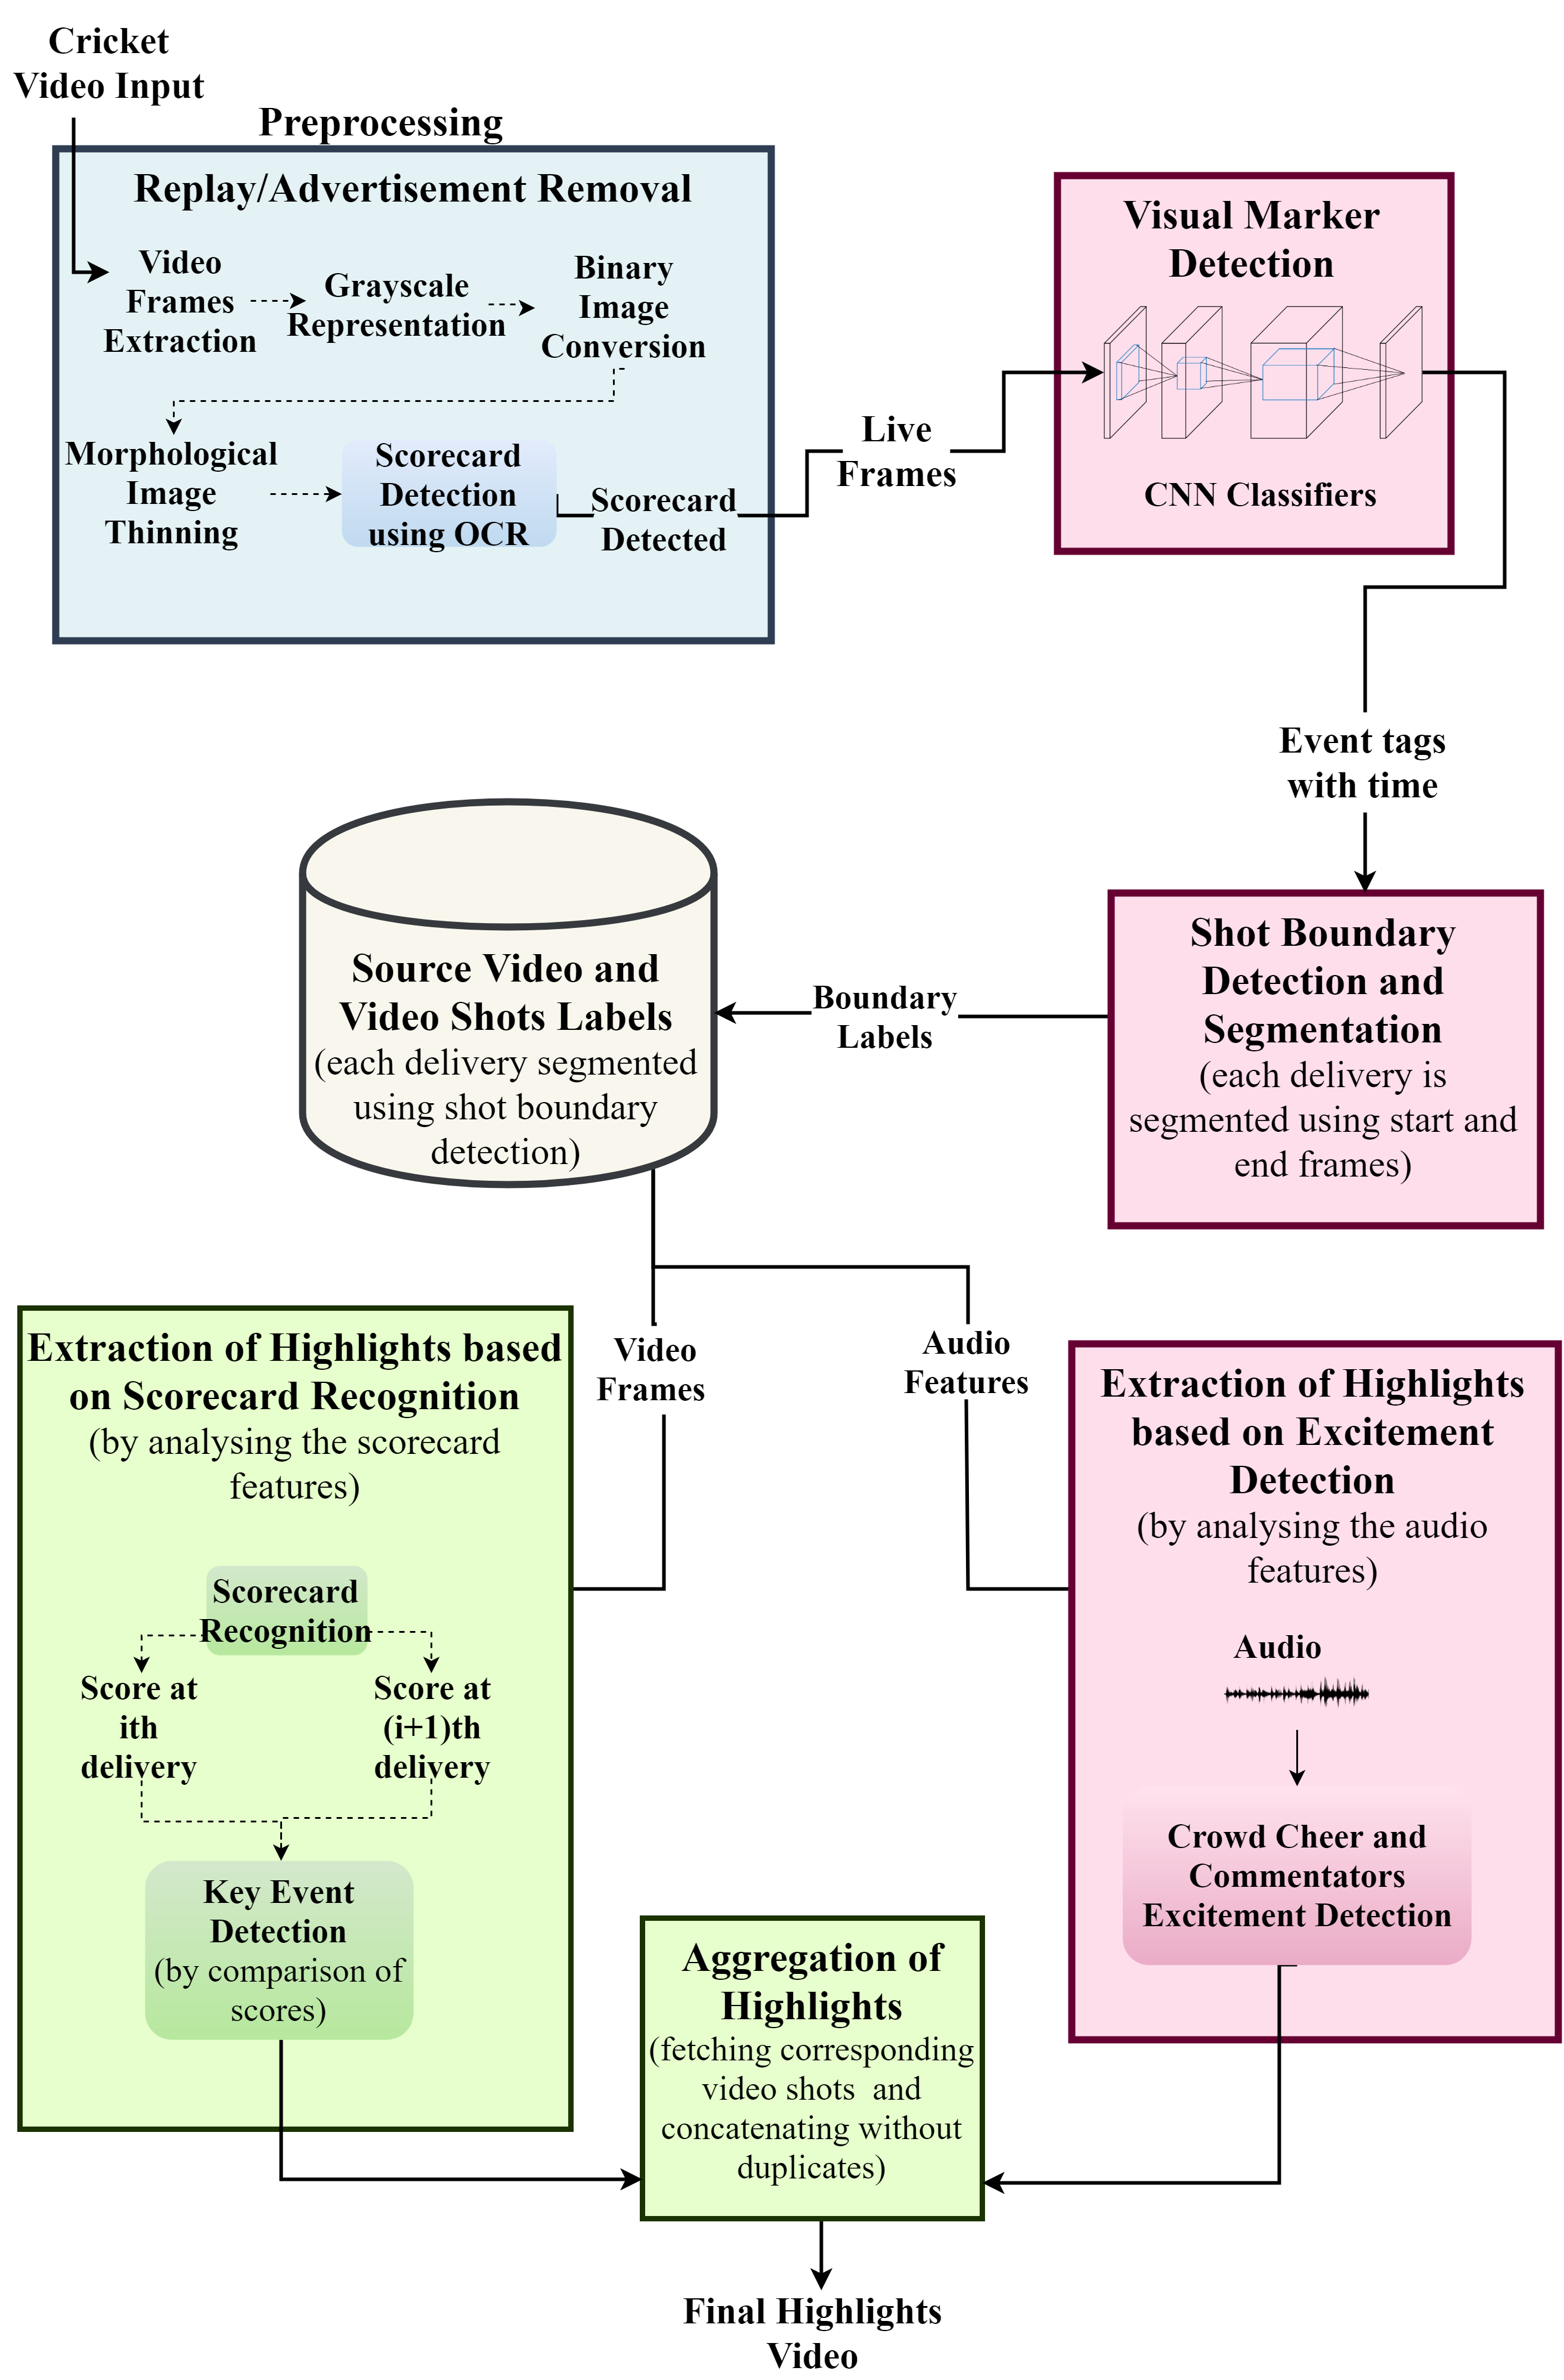
\includegraphics[width=0.9\textwidth,left]{Figures/SysArch.png}
    \caption{System Architecture}
    \label{fig:System Architecture}
\end{figure}
\newpage
\section {Module Design}
\subsection{Preprocessing}
Replays are the repetitive video shots of the key events in the cricket match. Advertisements are promotional video segments that are completly unrelated video shots for highlights extraction. Therefore, these shots are removed as they are considered to be unwanted. This module is used for detection and removal of replays and advertisements by checking the scorecard in the video frames. Absence and presence of the scorecard are used to detect replay/advertisement frames and live frames, respectively. The source video is converted into frames. In order to reduce the ambiguity for the OCR to detect the scorecard captions accurately we convert each frame into a morphed image. First, the frames are converted to gray scale representation which wont have any colours. Then it is converted to binary image. The brightness and contrast of each frame are increased slightly in order to represent the contour of the captions more precisely. OCR detects and recognizes the scorecard from each frame. Live frames are those which has scorecard are classified and are given to visual marker detection for event classification. Figure \ref{fig:preprocessing} shows the preprocessing of the input video.
\begin{figure}[h]
    \centering
   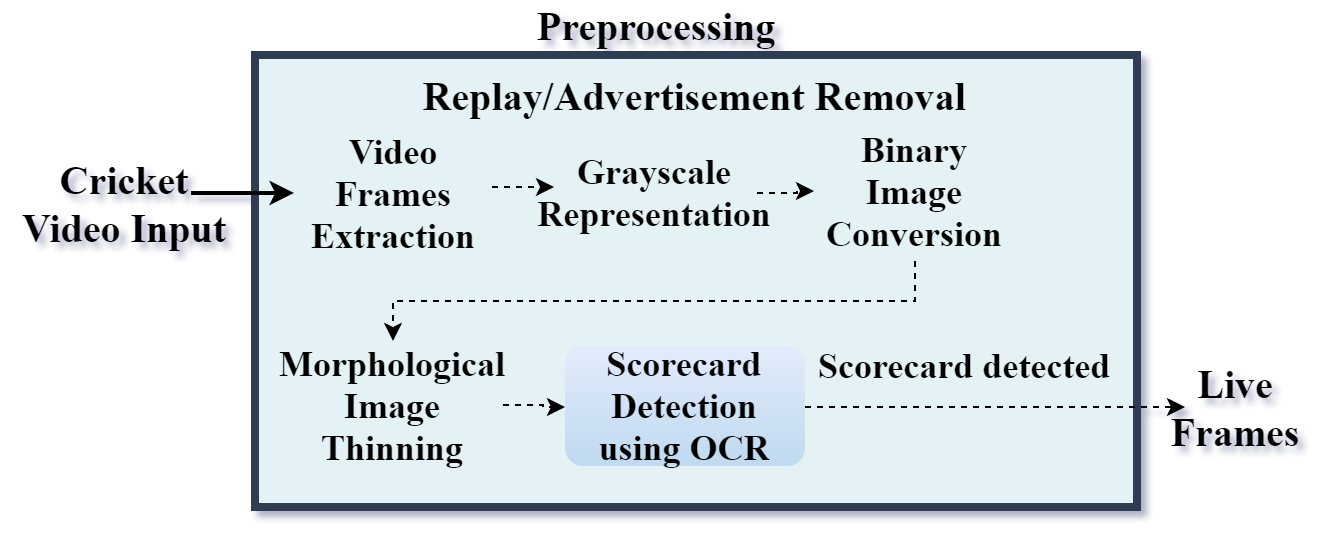
\includegraphics[width=1.0\textwidth,center]{Preprocessing.png}
    \caption{Workflow of Preprocessing}
    \label{fig:preprocessing}
\end{figure}

\newpage
\subsection{Visual Marker Detection}
Event detection and classification is important for shot boundary detection and segmentation. Visual marker detection detects events like batting, bowling, crowd, interviews, commentators etc. from the live frames using trained CNN classifiers. The Multiple classes present in the video are pitch view, commentators, interview, field view, crowd, closeup, players gathering, long shot and other undefinable classes. In order to reduce the dimension of the multi class classification problem in detecting the events accurately, ensemble classifiers  are used. The One vs All scheme\cite{Galar:2011:OEM:1963661.1963815} is used here. The complexity of multi class classification is compensated by binarization strategy. The classifier is trained with more than 4000 images with each class containing the training and testing images in the range of 300 and 100 respectively. The trained models are loaded to predict these  classes. The image is given to each classifier until it gets the positive output from a classifier. Each negative outputs of the classifier is subjected to the remaining classifiers. If all the classifier gives negative output, the frame is marked as unlabeled. The event tag along with the time of the event is given to the shot boundary detection and segmentation for grouping the frames into video segments. Layout of this module is shown in the figure \ref{fig:Visual Marker Detection}.

\begin{figure}[h]
    \centering
   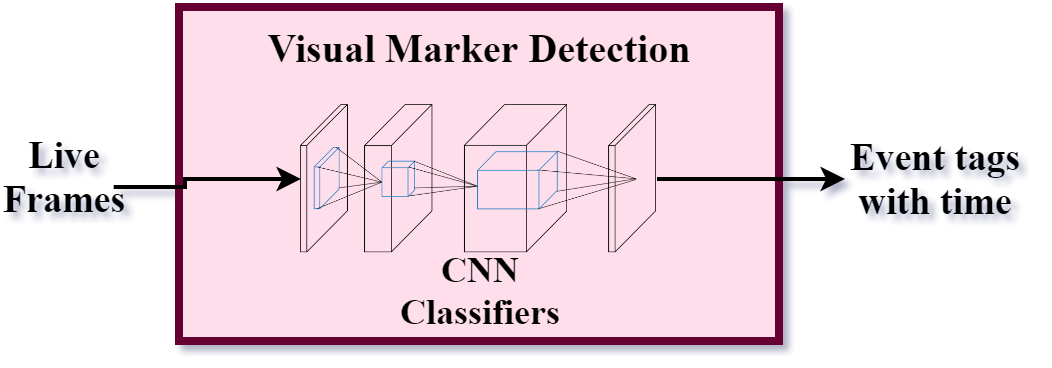
\includegraphics[width=1.0\textwidth,center]{VisualMarkerDetection.png}
    \caption{Workflow of Visual Marker Detection}
    \label{fig:Visual Marker Detection}
\end{figure}

\newpage
\subsection{Shot Boundary Detection and Segmentation}
Each ball starts with a pitch view where a bowler who runs from the pavilion end, bowls the ball and at the other end batsman will be in position to hit the ball. This event is marked as the start boundary of a ball(video segment). The events like crowd view, commentators view, interviews shot are shown in a cricket video only during the normal time i.e they are uninteresting parts of the video. The start frame of a ball shot segment can be identified by using the frames annotated with the label as pitch view or bowling view. The end boundary is identified by variety of strategies. 1) Once the start boundary is identified, the subsequent frames starting from the start frame are checked for the labels crowd view, commentators, interviews, field view. If the frame with above labels are seen, then that frame will be marked as the end boundary of that ball shot segment. 2) When the replay or advertisement is started before detecting the boundary labels, then that is marked as the end boundary of that ball shot segment. Then the following frames are checked to detect the next ball's start boundary and the process goes on until it reaches the end of the video. Using start and end of the delivery, shots are identified and segmented. The labels containing start and end time of the delivery is stored for further use in the following modules. Figure \ref{fig:ShotBoundaryDetection} shows the layout of the shot boundary detection.

\begin{figure}[h]
    \centering
   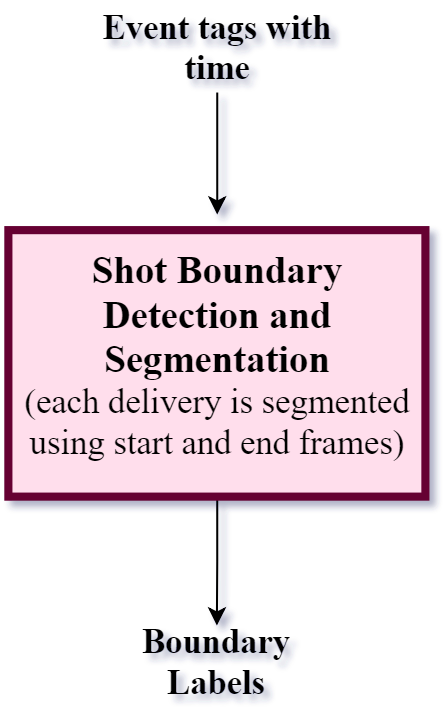
\includegraphics[width=1.0\textwidth,center]{ShotBoundaryDetection.png}
    \caption{Workflow of Shot Boundary Detection and Segmentation}
    \label{fig:ShotBoundaryDetection}
\end{figure}
\newpage
\subsection{Extraction of Highlights based on Scorecard Recognition}
It has been observed that the key events in the cricket video are mostly the events that involves fours, sixes and wickets. The scorecard captions contains the score (i.e the combination of runs and wickets) in that particular time, overs, two batsman's name with their score and some other necessary tags associated in that frame. Each frame is cropped to the bottom left part, in order to recognize the score of that particular frame. By using the above mentioned approach the score of the start frame of each video shot segments are recognized from the cropped image using OCR. The difference of the score from the start frame of current video shot segment and the start frame of the next shot is calculated. If run difference exceeds 4, then it is added to highlights or if the wicket difference exceeds 0 then that video shot segment is labeled as highlights. Corresponding delivery labels are given as the output to the next module. Figure \ref{fig:Scorecard} shows the layout of the extraction based on scorecard recognition module.

\begin{figure}[h]
    \centering
    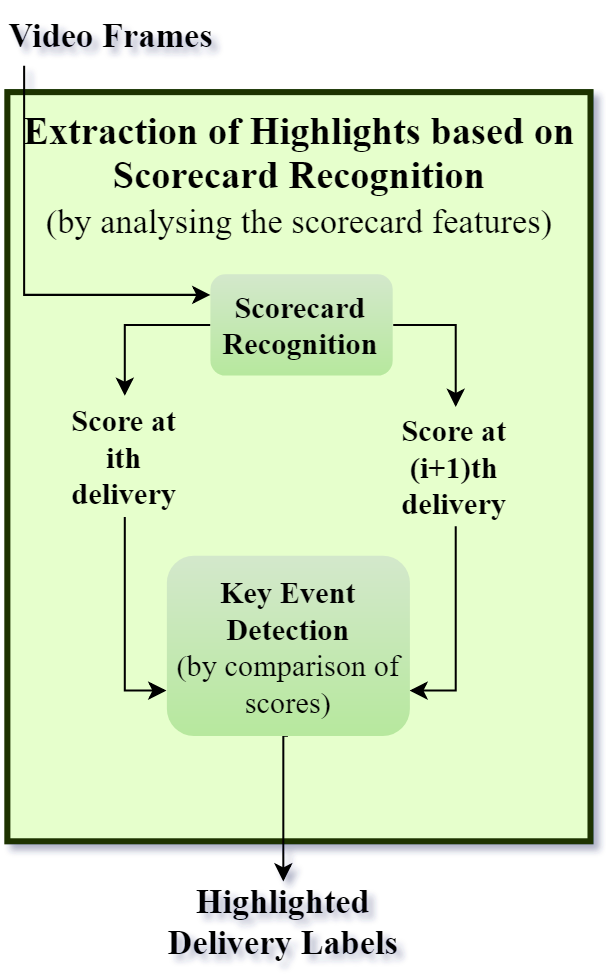
\includegraphics[width=1.0\textwidth]{Scorecard.png}
    \caption{Workflow of Extraction of Highlights based on Scorecard Recognition}
    \label{fig:Scorecard}
\end{figure}

\newpage
\subsection{Extraction of Highlights based on Excitement Detection}

Most of the key events in sports especially cricket will have crowd cheers and commentators excitement in that segment. This module is used for extracting highlights based on excitement using crowd cheer and commentators excitement from audio. The short time audio energies are used to detect the cheers and excitement. The short time audio energy in a time is computed by calculating the mean of the sum of the squares of all audio sample in that time. The short time audio energies of the whole video are calculated. The average of the short time audio energy for each time with the sliding window of length 5s is calculated. Normalized audio energy $NE$ at a time is calculated by finding the ratio of audio energy at that time to the maximum audio energy present in the video. Then $P_{audio}$ is calculated by finding the mean of the normalized audio energies. Now for each video segments $\Psi(n)$  is calculated by checking NEs with the $P_{audio}$. The mean of $\Psi$ for each ball shot segments are calculated. The threshold for excitement for the input video is set to the sum of the mean and variance of mean of $\Psi$ . A ball segment contains excitement if its mean of $\Psi$ exceeds the thresold and are classified as highlights. Corresponding labels of the shots are considered as the highlights and given to the next module.
Figure \ref{fig:Excitement} shows the layout of the extraction based on excitement detection module.

\begin{figure}[h]
    \centering
    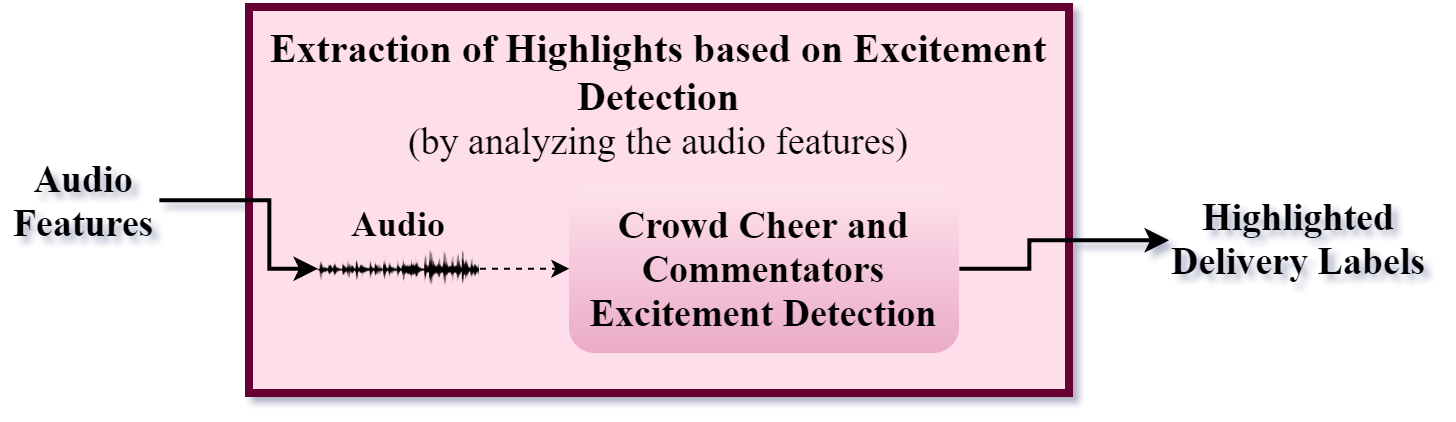
\includegraphics[width=1.0\textwidth]{ExcitementDetection.png}
    \caption{Workflow of Extraction of Highlights based on Excitement Detection}
    \label{fig:Excitement}
\end{figure}

\newpage

\subsection{Aggregation of Highlights}
The two lists from the previous modules contains the ball shots labels which are classified as highlights based on scorecard recognition and excitement detection respectively. Each ball label is checked for its presence in either of the lists or both. If the ball is present in any of those lists, then it is added to final highlights list. The final list is the combination of the two given lists without duplicates. The corresponding video shots for each highlight labels are fetched from the database by using the start and end boundary labels of those ball labels. The extracted video clips which are marked as highlights are then concatenated to generate the final highlights video. The final highlights video is the summarized version of the input cricket video which has the key events based scorecard recognition and excitement detection. Figure \ref{fig:Aggregation of Highlights} shows the layout of the aggregation.
\begin{figure}[h]
    \centering
    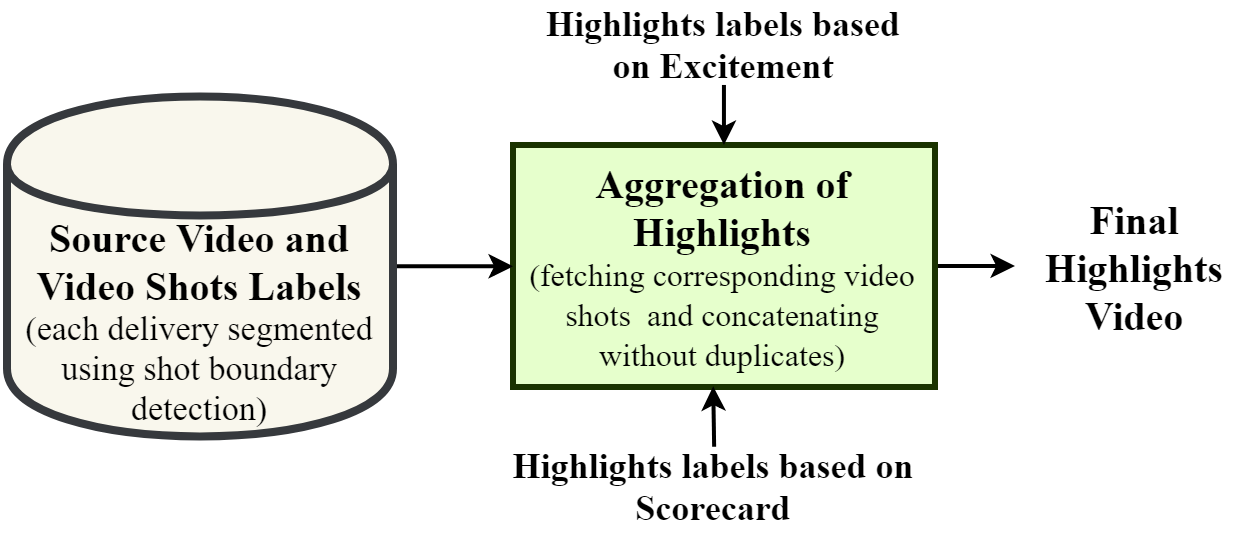
\includegraphics[width=1.0\textwidth]{Aggregation.png}
    \caption{Workflow of Aggregation of Highlights}
    \label{fig:Aggregation of Highlights}
\end{figure}

\newpage
\section{Complexity Analysis}
\subsection{Time Complexity}
Time complexity of each module of the system is shown in table \ref{tab:timecomplexity}.
\begin{table}[ht]
\caption{Time complexity of various modules} % title of Table
\centering 
\begin{tabular}{lll} 
\hline
S. No. & Module  & Complexity \\ [0.5ex] % inserts table
\hline
1 & Preprocessing &  $O(t\textsubscript{ocr})$   \\
2 & Visual marker detection &  $O(Nt_{c})$ \\
3 & Shot boundary detection and segmentation &  $O(T)$ \\
4 & Extraction of highlights based on scorecard recognition &  $O(B)$  \\
5 & Extraction of highlights based on excitement detection &  $O(T+B)$ \\
6 & Aggregation of highlights & $O(t_{aggr}t_{out})$\\[1ex]
\hline 
\end{tabular}
\label{tab:timecomplexity}
\end{table}
\begin{itemize}
    \item T is the duration of the input video
    \item t\textsubscript{ocr} is the computation time for OCR to detect scorecard in one frame
    \item t\textsubscript{class} is the run time of each classifier
    \item t\textsubscript{aggr} is the aggregation time for generating 1s video output
    \item t\textsubscript{out} is the duration of output video  in seconds
    \item N is the number of classifiers
    \item B is the number of ball shot segments present in the input
\end{itemize}
\subsection{Complexity of the project}
\begin{itemize}
    \item The accuracy of the system lies in event tagging, shot segmentation.
    \item The accuracy of the shot boundary detection depends on the classifier and the replay/advertisement removal. Shot boundary segmentation can wrongly segment if any frame is falsely classified as start of the ball
    \item Milestones are also an important event which cannot be identified by scorecard. Hence excitement is used to identify such key event.
    \item The accuracy of the output depends on shot boundary detection and segmentation. Error in this segmentation may leave out certain key event. So care should be taken in segmenting the shots.
    \item The efficiency of the visual marker detection also plays an important role. If the start of the ball is wrongly classified as the other frames or other frames classified as the start of the ball causes error in the outptut.   
\end{itemize}